\section{The uComp Protege Plugin - GW}


% T1. Verification of Domain Relevance.  Is a concept/instance relevant for a domain?
% T2. Verification of Relation Correctness. Does a certain relation between two ontology entities hold? These could be a set of generic relations (sameAs, subClassOf, instanceOf), but also arbitrary named relations to be specified by the ontology engineer. The crowd here would have to vote (yes/no) for a given triple (Subject - Relation - Object). This task is the focus of [1].
% T3. Learning of Relation Names. This is also a very difficult task in OL in general - the workers are presented with two terms and can choose between a set of given relations what applies. These relations can be a set of OWL relations that all ontologies have as well as a (restricted) number of domain specific relations specified by the expert (e.g., ÒinfluencesÓ). [BTW, since this is a complex task it could be split up into a sequence of 3 simpler tasks: 1) given two terms workers agree whether these are related or not; 2) those pairs that were judged related are then passed to another task where a correct relation is selected; 3) in the third task, the quality of the relations is checked - practically T2]

This section describes the actual plugin, ie.~which tasks have been implemented, the features and plugin usage. 
Protege was programmed in Java, it can easily be extended in the form of \emph{plugins} which are typically Java Archive (.jar) files
stored in the Protege plugin directory. The most common form of a Protege plugin is a view plugin, which implements a single view for a specific area of an ontology (e.g. classes, individuals, object properties, \dots).
%Florian: Protege completely was programmed in Java, therefore all plugins also are programmed in Java. Since Protege was developed very modular, it is quite easy to create simply plugins and integrate them into Protege. 
%Florian: All Protege plugins are so called jar-Files (Java Archive), and contains the compiled source code and all needed libraries. The most common form of a Protege plugin is a view plugin, which implements a single view for a specific area of an ontology (e.g. classes, individuals, object properties, ...)

% installation / SETUP 
Installation and setup
* The plugin is available at \url{TODO -- add link once uploaded to Protege}, includes detailed documentation about the tasks and 
the usage of the plugin. TODO (if necessary) documentation is accessible at ..
To use the plugin you need to your uComp-API key\footnote{Request a key from the uComp team, see \ur{http://soc.ecoresearch.net/facebook/election2008/ucomp-quiz-beta/api/v1/documentation/}} in a file named \texttt{ucomp\_api\_key.txt} in folder \texttt{.Protege}.
* Use an existing CF account key .. describe how to use it (place in conf file?!)
%Florian: The CF key has to be associated with the uComp-API key, therefore it has to be communicated to the uComp-API team (see http://soc.ecoresearch.net/facebook/election2008/ucomp-quiz-beta/api/v1/documentation/)
%Florian: The uComp-API key itself must be put into a textfile named "ucomp_api_key.txt" at the users home directory, in the folder ".Protege" (which is created by Protege during installation on both Windows and Linux plattforms) 

% PERSISTENCE 
 All data collected by the plugin which should be persistent is stored in the ontology in \texttt{rdfs:comment} fields,
for example information about the domain, the job ID, and results from the game.
%Florian: all information about the task is stored (depends on the kind of task): domain, validation of whole subtree going on?, additional information, sent to crowdflower or ucomp-quiz, ucomp-api job-id, ...

% give an example SCREEENSHOT with a quick introduction 
\begin{figure*}[htb]
\centering
{\centering \resizebox*{1.0\textwidth}{!}{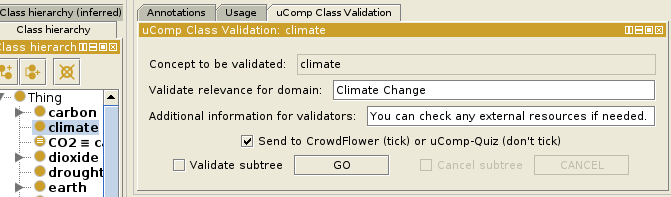
\includegraphics{images/c_rel_check_start.png}}}
 \caption{\label{fig:screen_cr}Screenshot showing the interface for validating a concept.}
\end{figure*}

Figure~\ref{fig:screen_cr} shows the basic interface for the domain relevance task, the other tasks
have similar interface.
Initially, the user adds the new view in the Protege window. The plugin interface contains 
task specific information (eg. the concept selected by the user for validation), 
generic information such as the \emph{domain} of the ontology and \emph{additional information} (see below),
and a \texttt{GO} button start the validation process.


% The common PROCESS 
The process itself is similar for all types of evaluation: (i) the user selects which part of the ontology 
should be verified (eg. a specific concept or all concepts), (ii) a requested is sent to the uComp API, 
(iii) as soon as available, the uComp API presents the results and saves them in the ontology.


% COMMON FIELDS in the UI: domain and additional information
What is common among all tasks handled by the plugin, is the selection of a ``domain'' and that the user can provide
additional information about the task. The domain is simply the field of knowledge which the ontology covers. If entered
once, the domain will be stored in the ontology (as \texttt{rdfs:comment}) and be pre-filled subsequently, but it can also be changed at any time.
For every task, the plugin contains a predefined task description (typically including examples) which is presented to the HC user.
If the ontology engineer wants to extend this task description, he or she can provide more guidelines 
in the field ``additional information''.
TODO: a few words about: validate subtree (only for tasks: concept relevance, subtree validation, TODO)
%Florian: domain will be stored as rdfs:comment in the head of the ontology


% USAGE 
In a nutshell, the user selects the part of the ontology to validate and optinally gives some additional information (see below). 
The plugin sends the request to the HC API (uComp API), which delegates the task to a GWAP or CrowdFlower. 
After enough HC users given their input on the task, the results are sent back to the plugin, which then displays them to the Protégé user. Depending on the result, the user can perform further actions like deleting negatively validated parts of the ontology.
* Explain: With plugins to Protege --> typically additional options in the Windows->Views Menu. 
  So in general, first open an ontology, then select the part of the ontology to verify (eg. the ``classes''), and finally 
  added the verfication frame via the Windows->Views menu.


% TODO -- describe TASKs
Task 1 - Verification of Domain Relevance.
* Being in class view, select the "uComp Class Validation" from the Windows->Views menu. 

into Windows->Views->class view. Add the 

